\documentclass[aps,prd,twocolumn,10pt,superscriptaddress,nofootinbib,longbibliography,floatfix]{revtex4-2}

\usepackage{amsmath,amssymb,amsfonts}
\usepackage{bm}
\usepackage{graphicx}
\usepackage{xcolor}
\usepackage{hyperref}
\graphicspath{{figures/}}
\hypersetup{colorlinks=true,linkcolor=blue,citecolor=blue,urlcolor=blue}

\newcommand{\dd}{\mathrm{d}}
\newcommand{\Kn}{\mathrm{Kn}}
\newcommand{\vM}{v_{\text{M\o l}}}
\newcommand{\sigmam}{\sigma_m}
\newcommand{\sigt}{\tilde\sigma}

\begin{document}

\title{Relativistic collapse of a self-interacting dark-matter core:\\ Scope, set-up, and baseline tests (working note v1)}

\author{Track C of the numerical-relativity particle-in-cell cosmology program}

\date{Working note v1, state of 21 November 2026}

\begin{abstract}
When the core of a halo of self-interacting dark matter has conducted its heat outward for long enough, it contracts until its particles move close to the speed of light and it falls into a black hole. How much of the core ends in the black hole is known only from spherical fluid models, whose closure fails where the mean free path of the particles grows. This working note scopes a calculation that answers the question with collisionless particles coupled to numerical relativity in three dimensions, extended by a relativistic Monte Carlo collision operator, so that one number, the Knudsen number, moves the core from the collisionless to the fluid regime, and it records the baseline tests of that operator. Real cores have Knudsen numbers twelve to twenty orders of magnitude below what particles can resolve, so the planned scan is a bridge between the two limits, anchored at the fluid end by the exact pulsation onset of the same equilibrium. With the adiabatic index of a collision-dominated relativistic gas, that onset lies just on the stable side of the turning point of the binding energy, for the King family and for the thermal core of the scan alike. In a periodic box the operator conserves energy and momentum to rounding, collides at the relativistic rate from cold to ultrarelativistic temperatures, keeps that rate in a static curved metric, streams freely at long mean free path, and at short mean free path conducts heat with the Chapman--Enskog conductivity of hard spheres, at relativistic temperatures as well. The first King clusters evolved with collisions contract relative to their collisionless twins and collapse; the drift of the collisionless twins on the mesh used is larger than the stability margin, so these scouting runs leave the collisional threshold open.
\end{abstract}

\maketitle

\section{Introduction}\label{sec:intro}

Dark-matter particles that scatter elastically off each other conduct heat inside a halo. A self-gravitating core has a negative heat capacity: when it loses heat to the halo around it, it contracts and becomes hotter, so the heat flow continues and the core runs away in a gravothermal collapse \cite{Balberg:2002gt,Koda:2011sidm}. The collapse ends when the velocity dispersion of the core approaches the speed of light and general relativity makes the core dynamically unstable \cite{Balberg:2002bh,Feng:2021instab}. The black hole that forms is a candidate seed for the massive black holes that the James Webb Space Telescope finds early in cosmic history \cite{Feng:2021seed,Feng:2025lrd,Shen:2025lrd}, so the fraction of the core that ends in the black hole matters for that interpretation.

The estimates of this fraction come from fluid models. A conducting fluid follows the gravothermal phase and agrees with Monte Carlo $N$-body simulations in the transitional regime of mean free paths \cite{Koda:2011sidm}, and a spherically symmetric kinetic code follows the late collapse beyond the fluid approximation \cite{Gurian:2025sidm}. Equilibria of a truncated thermal distribution give the onset of the relativistic instability through the turning point of the binding energy and through an adiabatic criterion for radial pulsations \cite{Feng:2021instab}. The only time-dependent relativistic calculation is a spherical fluid with heat flux in the Misner--Sharp form, which follows the core to horizon formation and finds a black hole that holds a tiny fraction of the halo \cite{Gu:2026sidm}; its authors point out that a rigorous treatment requires the collisional Boltzmann equation \cite{Gu:2026sidm}. For collisionless relativistic clusters the turning point of the binding energy marks the onset of instability of the King and polytropic families, and the collapse then takes every particle into the black hole \cite{Gunther:2020ev}; core--halo families can stay stable beyond the first turning point \cite{Gunther:2021ev}.

This track computes the collapse with particles. The numerical-relativity particle-in-cell method of Wu and Most \cite{Wu:2026nrpic} evolves macroparticles on geodesics together with the spacetime and has followed relativistic clusters through their instability. Here the method, rebuilt in the code AthenaK, gains a relativistic Monte Carlo collision operator, so that a single dimensionless number, the Knudsen number of the core, moves the matter from the collisionless regime to the collision-dominated one. The relaxation time of a real core exceeds its dynamical time by many orders of magnitude, so the runs start from an equilibrium close to the instability threshold. The work is carried out by large-language-model agents under human direction.

This note records the scoping stage and the baseline tests:
\begin{itemize}
\item the Knudsen numbers of real cores lie far below anything that particles can resolve, so the planned scan is a bridge between the collisionless and the fluid limits, anchored at the fluid end (Sec.~\ref{sec:knudsen});
\item along the thermal-core sequence the turning point of the binding energy and the fluid pulsation onsets separate, and the closure of the fluid decides where its onset sits (Sec.~\ref{sec:t-sequences}); with the index of a collision-dominated gas the onset lies just on the stable side of the turning point in both families (Sec.~\ref{sec:t-onsets});
\item the references of the collision operator agree with independent checks, the code's collision kernels reproduce exact test vectors, and the code moves particles exactly in a collisionless periodic box (Secs.~\ref{sec:t-collisions} and \ref{sec:t-box});
\item in the box the operator conserves four-momentum, collides at the relativistic rate also in a static curved metric, and its energy can be conserved at each particle's own metric (Sec.~\ref{sec:t-operator});
\item the operator conducts heat with the Chapman--Enskog conductivity of hard spheres, at relativistic temperatures as well (Sec.~\ref{sec:t-heat});
\item the first King clusters with collisions contract relative to their collisionless twins and collapse, within limits that the mesh and a single seed set (Sec.~\ref{sec:t-clusters}).
\end{itemize}
Section~\ref{sec:problem} states the problem, Sec.~\ref{sec:setup} the set-up and the numerical methods, Sec.~\ref{sec:tests} the tests, Sec.~\ref{sec:g2} the collisionless threshold toward the capability gate, and Sec.~\ref{sec:plan} the plan to the next gates and what is open. Table~\ref{tab:parameters} holds the parameters of the equilibrium models, and Tables~\ref{tab:ledger}--\ref{tab:ledger4} every number of the note with the registered run that produced it.

\section{From gravothermal collapse to a relativistic instability}\label{sec:problem}

\subsection{Two clocks}\label{sec:clocks}

Two times govern the core. The relaxation time, the time for collisions to carry heat across the core, sets the pace of the gravothermal collapse. The dynamical time, the free-fall time of the core, sets the pace of the relativistic instability. In the fluid calculation of Ref.~\cite{Gu:2026sidm} even the fastest phase of the collapse lasts tens of thousands of dynamical times of the core, and the approach to the horizon far longer (Table~\ref{tab:ledger2}). Following that history step by step at the resolution of the dynamical time is out of reach. The calculation therefore starts from an equilibrium core close to the threshold of the relativistic instability and asks what happens next, with the collisions switched on at a chosen strength.

\subsection{Equilibrium families}\label{sec:families}

A static, spherically symmetric, isotropic solution of the Einstein--Vlasov system has a distribution function $f$ that depends on the phase-space coordinates only through the Killing energy per unit rest mass, $E=-u_t$, which every particle conserves. Three families serve the track. The truncated thermal family has the thermal kernel
\begin{equation}\label{eq:kernel}
f(E)=A\left[\exp\!\left(\frac{1-E/E_c}{b}\right)-1\right]\quad (E<E_c),
\end{equation}
and $f=0$ above the cutoff energy $E_c$, where $A$ is a normalization and $b=k_BT(R)/m$ is the temperature at the edge $R$ in units of the particle mass $m$. Since the temperature follows the Tolman law, this kernel is the truncated Maxwell--Boltzmann distribution of Ref.~\cite{Feng:2021instab}, whose sequence at fixed $b$ is labelled by $w_0$, the central cutoff kinetic energy over the local temperature. A small $b$ gives a hot, dense core inside an extended envelope; we call the member with $b=0.1$ the thermal core, and it is the primary family of the scan, the one Ref.~\cite{Gu:2026sidm} uses for its onset. The member with $b=1$ is the King model of Ref.~\cite{Gunther:2020ev}, labelled by the central value $y_0$ of its potential variable. The monoenergetic family of Ref.~\cite{Wu:2026nrpic} gives every particle the same Killing energy and is labelled by $y_c$, the central value of the squared ratio of central to surface lapse. The King and monoenergetic families serve verification: their collisionless thresholds are known \cite{Gunther:2020ev,Wu:2026nrpic}.

Along each sequence the central redshift to infinity, written $Z(0)$ for the thermal core and $z_c$ for the other two families, grows monotonically, and the binding-energy fraction $\epsilon=(M_0-M)/M_0$, with $M_0$ the rest mass and $M$ the ADM mass, rises to a maximum and falls again. The central lapse is $\alpha_c=1/(1+Z(0))$. Table~\ref{tab:parameters} lists the models at the instability criteria of Sec.~\ref{sec:t-sequences}.

\subsection{The Knudsen number}\label{sec:knudsen}

The Knudsen number compares the mean free path of the particles with the size of the system. Following the gravothermal literature \cite{Balberg:2002gt,Gu:2026sidm} we take the mean free path $\lambda$ and the gravitational scale height $H$ at the centre,
\begin{equation}\label{eq:kn}
\lambda=\frac{1}{\rho_0\sigmam},\qquad H=\left(\frac{v_1^2}{4\pi\rho_0}\right)^{1/2},\qquad \Kn_c=\frac{\lambda_c}{H_c},
\end{equation}
where $\rho_0$ is the rest-mass density, $\sigmam$ the cross-section per unit mass, and $v_1^2=(p+2p_T)/(3\rho_0)$ the squared one-dimensional velocity dispersion built from the radial and tangential pressures $p$ and $p_T$. In code units, with $G=c=1$ and the ADM mass $M$ as the unit, the cross-section per unit mass becomes a number $\sigt$, and each equilibrium model has its conversion constant
\begin{equation}\label{eq:conversion}
\sigt\,\Kn_c=K\equiv\frac{1}{\rho_{0c}H_c}.
\end{equation}
The constant varies little across the particle models of the track [Fig.~\ref{fig:knudsen}(b), Tables~\ref{tab:ledger} and \ref{tab:ledger4}], and a factor fixed by the physical units turns $\sigt$ into centimetres squared per gram for a given core mass.

Figure~\ref{fig:knudsen}(a) places real cores on this scale. For the cross-sections favoured by halo observations, a core of the black-hole mass found by the fluid calculation \cite{Gu:2026sidm} has a central Knudsen number some twenty orders of magnitude below unity, and a core as massive as the seed of the quasar benchmark of Ref.~\cite{Feng:2021instab} still lies a dozen orders below. Real relativistic cores are perfect fluids on their dynamical time. Particles resolve a collision length only if each collision cell is smaller than the mean free path and holds enough particles, so the particle number grows as $\Kn^{-3}$; the planned scan covers central Knudsen numbers from a few tenths to a hundred. The scan therefore maps the bridge from the collisionless to the fluid limit, and every statement about real seeds goes through its small-$\Kn$ end, which we anchor with the exact pulsation onset of the same equilibrium treated as a fluid.

\begin{figure*}
\centering
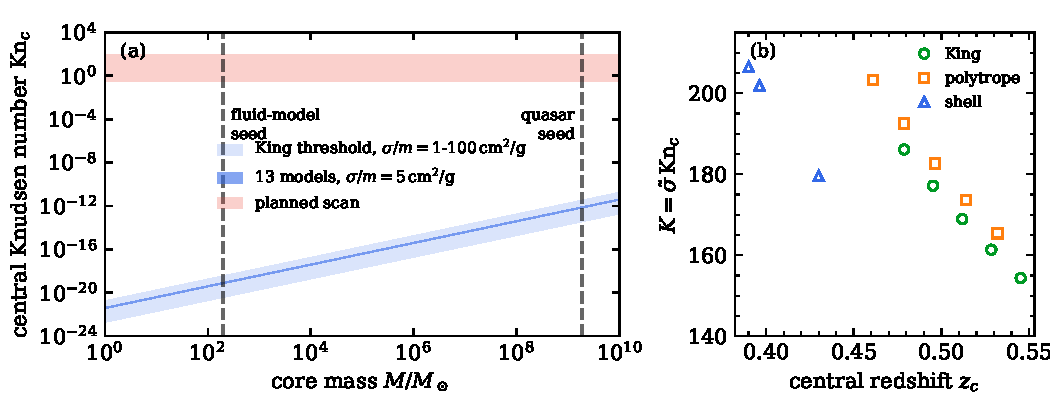
\includegraphics[width=\textwidth]{fig_knudsen.pdf}
\caption{Knudsen numbers of real cores and of the planned scan. (a) Central Knudsen number of the near-threshold models scaled to a core mass, for cross-sections per unit mass of $1$--$100\,$cm$^2$/g (light band, King threshold model) and $5\,$cm$^2$/g (dark band, all thirteen models); the red band is the planned scan, the dashed lines the black-hole mass of the fluid calculation \cite{Gu:2026sidm} and the seed of the quasar benchmark \cite{Feng:2021instab}. (b) Conversion constant of the thirteen particle models against their central redshift.}
\label{fig:knudsen}
\end{figure*}

\subsection{Observables}\label{sec:observables}

The track measures two things. The first is the collisionless instability threshold of each family, located with three-way convergence in particle number, cell size and domain size and compared with the turning point of the binding energy; for the King and monoenergetic families it reproduces the literature, for the thermal core it is new. The second is the collapsed mass fraction $f_{\rm BH}=M_{\rm BH}/M$, the mass of the apparent horizon at its formation and at the end of a run over the ADM mass, against the central Knudsen number, for thermal cores on both sides of the collisionless threshold and converged in particle number and collision step. Without collisions the King collapse takes every particle \cite{Gunther:2020ev}; whether a thermal core leaves its envelope behind, and how collisions change that, is the science question.

\section{Set-up and numerical methods}\label{sec:setup}

\subsection{The calculation}\label{sec:architecture}

The calculation has three parts (Fig.~\ref{fig:architecture}). The initial data are equilibrium models written as tables of the metric and as particle samples of the distribution function. The evolution couples the particles to the spacetime and adds the collisions. The analysis compares the runs with reference solutions computed outside the code: the collision rate, relaxation, conduction and entropy of a Maxwell--J\"uttner gas, the slab sums of a periodic box, a nonlinear isobaric conduction reference, and the radial-pulsation onset of each equilibrium. Every simulation capability lives in the one code; the track specifies what the code must do, supplies the reference solutions and tests, and checks the implementation. At the baseline gate the operator, its box tests, the particle models of both families and the fluid onsets exist; the energy convention at each particle's metric is an option of the code that was tested before it entered the code's release; the threshold scan, collisions on refined meshes and an energy diagnostic of the whole spacetime are still to come.

\begin{figure*}
\centering
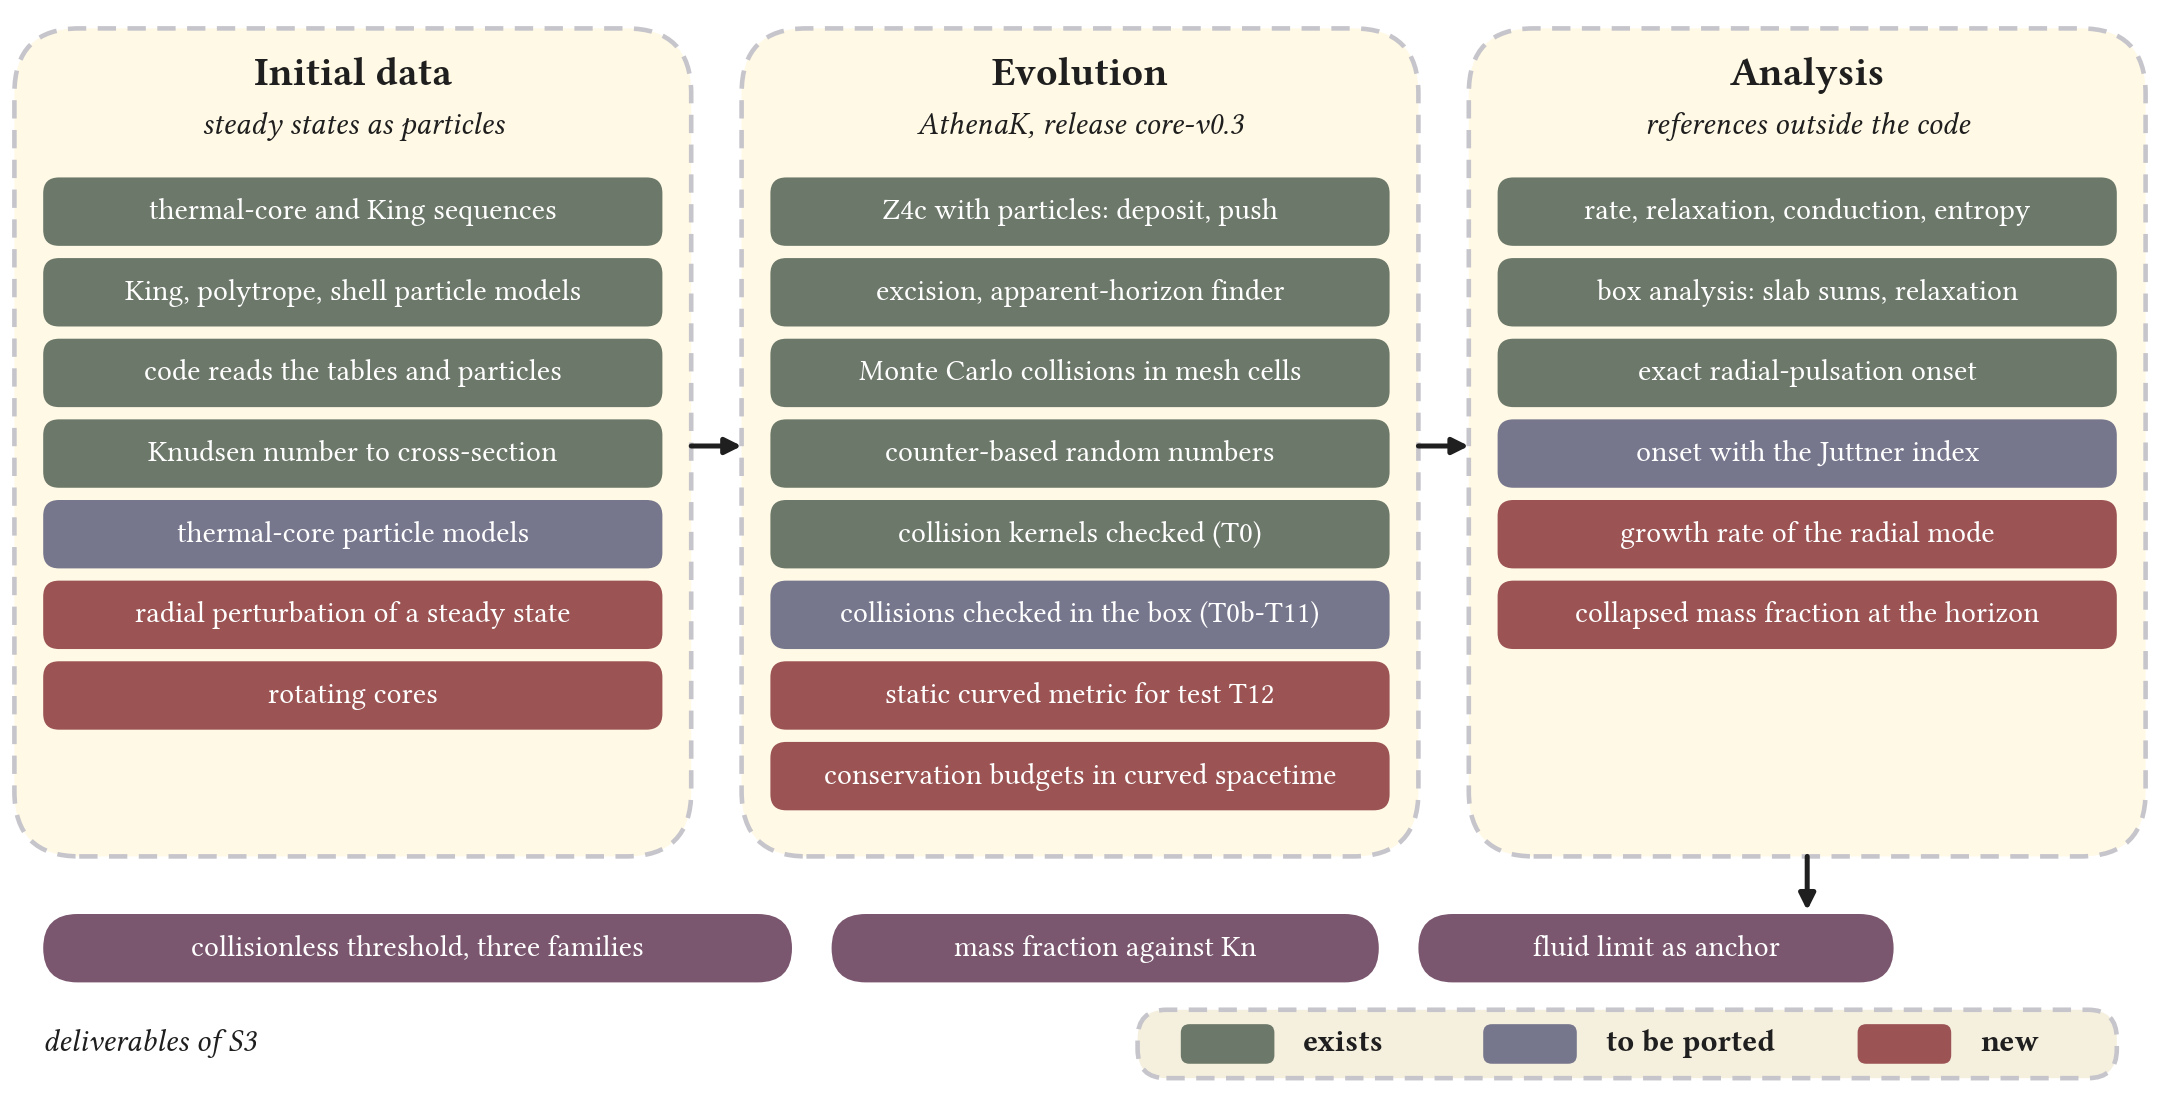
\includegraphics[width=0.92\textwidth]{schem_architecture.png}
\caption{Architecture of the calculation at the baseline gate. Green blocks exist and are tested, slate blocks exist as an option of the code or for another setting and are to be carried over, red blocks are still to be written. The purple pills are the deliverables.}
\label{fig:architecture}
\end{figure*}

\subsection{Relativistic Monte Carlo collisions}\label{sec:collisions}

Collisions are added by direct-simulation Monte Carlo in the cells of the mesh. Once per time step, after the particles have moved, the particles of each collision cell are paired at random. A tested pair $(i,j)$ collides with the pair probability
\begin{equation}\label{eq:pairprob}
P_{ij}=\frac{(N-1)\,\sigmam\,M_i\,\vM\,\alpha\,\Delta t}{\sqrt{\gamma}\,\Delta x\,\Delta y\,\Delta z},
\end{equation}
where $N$ is the number of particles in the cell, $M_i$ the rest mass of a macroparticle (all equal), $\alpha$ the lapse, $\gamma$ the determinant of the spatial metric at the cell centre, and $\Delta t$ and $\Delta x\,\Delta y\,\Delta z$ the coordinate step and cell volume, so that the denominator and $\alpha\Delta t$ are the proper volume and the proper time. The M\o ller speed of the pair,
\begin{equation}\label{eq:moller}
\vM=\frac{\sqrt{\gamma_{\rm rel}^2-1}}{W_iW_j},\qquad \gamma_{\rm rel}=-u_i\cdot u_j,
\end{equation}
with $W=(1+u^2)^{1/2}$ the Lorentz factor of each particle in the frame of the normal observer at the cell centre, makes the number of collisions per unit four-volume a Lorentz scalar. A pair that collides scatters elastically and isotropically in its centre-of-momentum frame. The pair conserves its four-momentum to rounding with the metric of the cell centre; as an option, it conserves the sum of its covariant momenta and of its canonical energies $\alpha W-\beta^iu_i$ with the metric at each particle, which matters where the metric varies across a cell. In the Newtonian limit the scheme reduces to the one of Koda and Shapiro \cite{Koda:2011sidm} with a cell as kernel. Each pairing, acceptance and direction draws its random numbers from a counter keyed by the seed, the step and the particle tags, so that a run gives the same particles for any division of the mesh among processors.

For a Maxwell--J\"uttner gas at temperature $\theta=T/m$ the same rule gives the M\o ller-averaged rate per particle,
\begin{equation}\label{eq:rate}
\Gamma=\rho_0\sigmam\langle\vM\rangle,\qquad \langle\vM\rangle=\frac{4K_3(2\zeta)}{\zeta K_2(\zeta)^2},
\end{equation}
with $\zeta=1/\theta$ and $K_\nu$ the modified Bessel functions of the second kind. At low temperature the average tends to $\sqrt{16\theta/\pi}$, the hard-sphere rate of the gravothermal literature \cite{Balberg:2002gt}; at high temperature it tends to unity. This M\o ller-averaged rate is the reference of the collision-rate test.

\subsection{Numerical methods}\label{sec:methods}

The spacetime is evolved in the Z4c formulation on the mesh of AthenaK, and the macroparticles move on geodesics of the evolving metric; their stress-energy is deposited on the mesh with cloud kernels, and an apparent-horizon finder with excision of its interior follows the black hole \cite{Wu:2026nrpic}. The cluster initial data are the equilibrium models in conformally flat isotropic coordinates, read as radial tables of the metric functions together with a particle file sampled from the distribution function. The collision step acts after the push on the particles that each mesh block owns, in the orthonormal frame of the normal observer at the cell centre, with the metric of the end of the step. The box tests use the flat metric, or a static metric with constant lapse $\alpha_0$ and conformal factor $\psi_0$, in a periodic domain, and the particle push alone.

\section{Tests and baseline results}\label{sec:tests}

\subsection{Equilibrium sequences and onsets}\label{sec:t-sequences}

The spherical baseline is an independent solver for each family. The thermal-core solver reproduces the two printed tables of Ref.~\cite{Feng:2021instab} row by row; the remaining differences are small, the radius column is printed coarsely, and three printed entries are misprints (Table~\ref{tab:ledger}). A second, independently written solver agrees with it to the level of the integration tolerances, and three solvers agree on the King sequence.

Figure~\ref{fig:sequences}(a) shows the binding-energy fraction of the thermal core with the printed rows. Three criteria mark the onset of instability along the sequence, in increasing central redshift: the maximum of the binding energy, the zero of the lowest squared radial-pulsation frequency $\omega_0^2$ of the same profile treated as a perfect fluid with the adiabatic index $\Gamma=1+p/u$ of Ref.~\cite{Feng:2021instab} ($u$ the thermal energy density), and the trial-function criterion of that reference. The pulsation onset comes from a Rayleigh--Ritz finite-element solution of Chandrasekhar's equation; on polytropes, where the zero must coincide with the maximum of the mass, it does so to the accuracy of the solver. Figure~\ref{fig:sequences}(b) shows how the onset moves with the closure: with $\Gamma=5/3$ the zero lies beyond the trial criterion. For the same adiabatic index the trial criterion is sufficient for instability, so the exact onset lies below it, as found. Reference~\cite{Feng:2021instab} reports its onset as insensitive to the trial function; for these centrally condensed models the exact onset lies well below the trial criterion, so the trial value marks a late bound on the onset, and an independent recomputation of the exact mode finds the same.

These criteria separate because they answer different questions. The turning point of the binding energy marks the collisionless onset of the King and polytropic families \cite{Gunther:2020ev}, while the pulsation onset is the threshold of a fluid whose collisions keep it in local equilibrium, and it depends on the adiabatic index. A core with a finite Knudsen number lies between these limits, and the scan measures where its threshold falls. For core--halo families the collisionless onset itself can move away from the turning point \cite{Gunther:2021ev}, so for the thermal core it is measured.

Figure~\ref{fig:sequences}(c) shows the two verification families. The King maximum reproduces the printed value of Ref.~\cite{Gunther:2020ev}, the monoenergetic maximum falls between the stable and the collapsing models of Ref.~\cite{Wu:2026nrpic}, and the five printed models of that reference are reproduced to their printed digits. The particle models built for the scoping stage (King and polytropic models on both sides of the turning point, and shells of Ref.~\cite{Andreasson:2006ev}) pass every offline check of their sampling and constraints.

\begin{figure*}
\centering
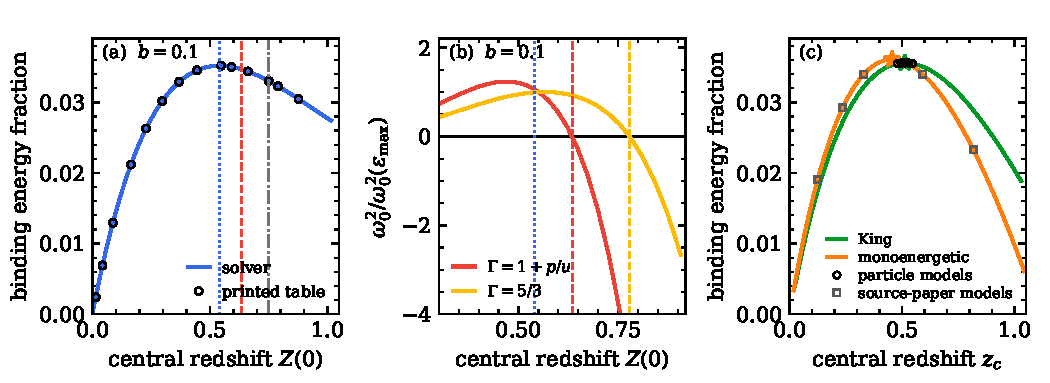
\includegraphics[width=\textwidth]{fig_sequences.pdf}
\caption{Equilibrium sequences. (a) Binding-energy fraction of the thermal core ($b=0.1$) against the central redshift, solver (line) and printed rows of Ref.~\cite{Feng:2021instab} (circles); vertical lines: binding-energy maximum (dotted), pulsation onset with $\Gamma=1+p/u$ (dashed), trial criterion (dash-dotted). (b) Lowest squared pulsation frequency, normalized at the binding-energy maximum, for two adiabatic indices; dashed lines at the zeros. (c) King and monoenergetic families with their maxima (stars), the particle models and the models of Ref.~\cite{Wu:2026nrpic}.}
\label{fig:sequences}
\end{figure*}

\subsection{The fluid anchor: onsets of a collision-dominated gas}\label{sec:t-onsets}

A gas whose collisions keep it in local equilibrium oscillates adiabatically with the first adiabatic index of a Maxwell--J\"uttner gas, $\Gamma_1=1+1/c_v$, where $c_v$ is the specific heat per particle at constant volume at the local temperature. The index falls from $5/3$ in the cold limit to $4/3$ in the ultrarelativistic one. This index, evaluated at the temperature that gives the local mean energy, defines the small-$\Kn$ anchor of the scan; the ratio of pressure to number density as the temperature gives nearly the same onset (Table~\ref{tab:ledger4}).

Figure~\ref{fig:onsets} shows the result for both families. With $\Gamma_1$ the pulsation onset lies just on the stable side of the binding-energy maximum, for the King family and for the thermal core alike, while the index $\Gamma=1+p/u$ places it far on the unstable side. The window in which collisions can move the threshold away from its collisionless value is therefore a narrow band of central redshift below the turning point: a King model at the collisionless threshold is unstable as a fluid, and a slightly less compact one is stable at both ends of the Knudsen scale. The two King models of the first collisional runs (Sec.~\ref{sec:t-clusters}) bracket the fluid onset.

Particle models of both families now exist at two particle numbers: five King models around the turning point and eight thermal cores from the stable side of the fluid onset to the onset with $\Gamma=1+p/u$ [Fig.~\ref{fig:onsets}(a,b)]. They pass the offline checks of their sampling and constraints, except three residual checks of the most compact thermal cores whose excess is the step error of the check itself (Table~\ref{tab:ledger4}).

\begin{figure*}
\centering
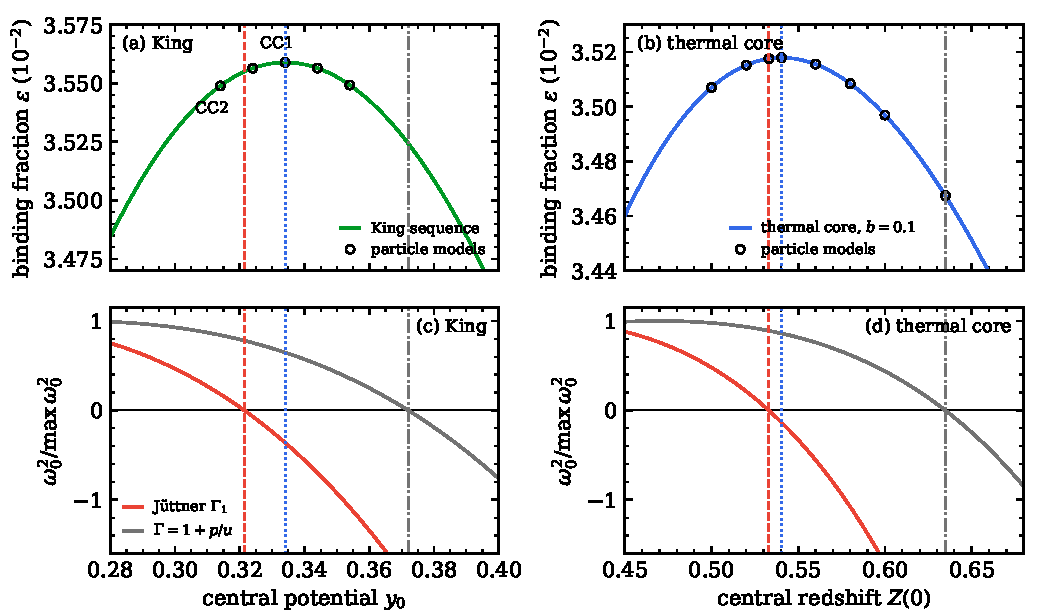
\includegraphics[width=\textwidth]{fig_onsets.pdf}
\caption{Collisionless and fluid onsets. Top: binding-energy fraction near its maximum, (a) King family against its central potential, (b) thermal core ($b=0.1$) against its central redshift, with the particle models (circles) and the models CC1 and CC2 of the first collisional runs. Bottom: lowest squared pulsation frequency, normalized by its largest value, for the J\"uttner index $\Gamma_1$ and for $\Gamma=1+p/u$. Vertical lines: binding-energy maximum (dotted), $\Gamma_1$ onset (dashed), $1+p/u$ onset (dash-dotted).}
\label{fig:onsets}
\end{figure*}

\subsection{Collision references and kernels}\label{sec:t-collisions}

The collision operator was specified before it existed in the code, with references independent of the code. Figure~\ref{fig:collisions}(a,b) compares the M\o ller-averaged rate with a three-dimensional quadrature over both momenta that bypasses the reduction to one integral: the two agree to the resolution of the quadrature at all temperatures. Monte Carlo averages over independently sampled pairs reproduce the rate, the exact relaxation rate of two populations at different temperatures, and the entropy estimator within two standard errors [Fig.~\ref{fig:collisions}(c)]. The relaxation of a hot gas is far slower than its non-relativistic form predicts (Table~\ref{tab:ledger2}). The rate and covariance tests are designed so that a code using the difference of the three-velocities in place of the M\o ller speed fails them.

The code's collision kernels were then fed exact test vectors, pairs whose expected outcomes were computed in sixty-digit arithmetic over many decades of temperature and bulk Lorentz factor. Under three compiler settings every case passes: the largest error of a post-collision velocity is a small fraction of its tolerance, and the four-momentum of each pair is conserved to about one unit roundoff [Fig.~\ref{fig:collisions}(d)]. Two independently written drivers of this test agree.

\begin{figure*}
\centering
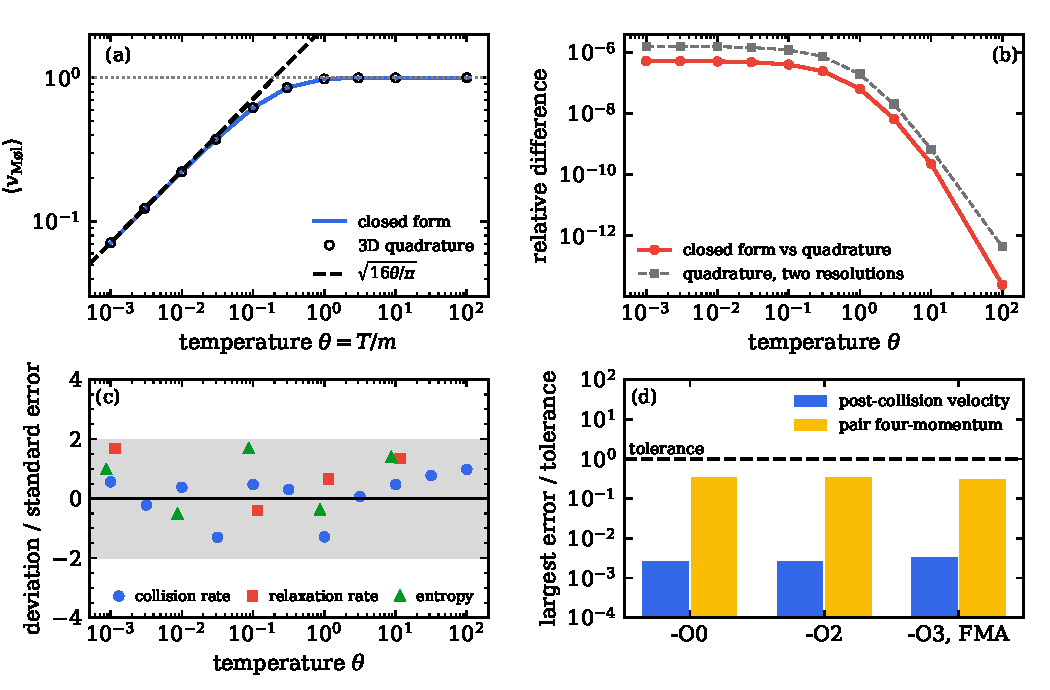
\includegraphics[width=0.9\textwidth]{fig_collisions.pdf}
\caption{References of the collision operator and the kernel test. (a) M\o ller-averaged speed of a Maxwell--J\"uttner gas, closed form (line) and three-dimensional quadrature (circles), with the low-temperature limit (dashed). (b) Relative difference of the two, and of the quadrature at two resolutions. (c) Monte Carlo checks in units of their standard error; grey band: two standard errors. (d) Largest error of the code's kernels over the test vectors, as a fraction of its tolerance, for three compiler settings.}
\label{fig:collisions}
\end{figure*}

\subsection{Particles in a periodic box}\label{sec:t-box}

The box tests of the collision operator start from the collisionless limit, which has an exact solution. Two slabs of a periodic Minkowski box hold Maxwell--J\"uttner gases at equal pressure and different temperatures; without collisions every particle streams on a straight line, and the mass and energy in the left slab follow a closed form for an infinite sample. Figure~\ref{fig:box} shows the code's slab sums: they equal those of straight-line streaming of the same sample to rounding, the positions agree with it to rounding, and both follow the ensemble curve within the sampling noise. The analysis of the box tests is thereby checked on the code's own output.

\begin{figure*}
\centering
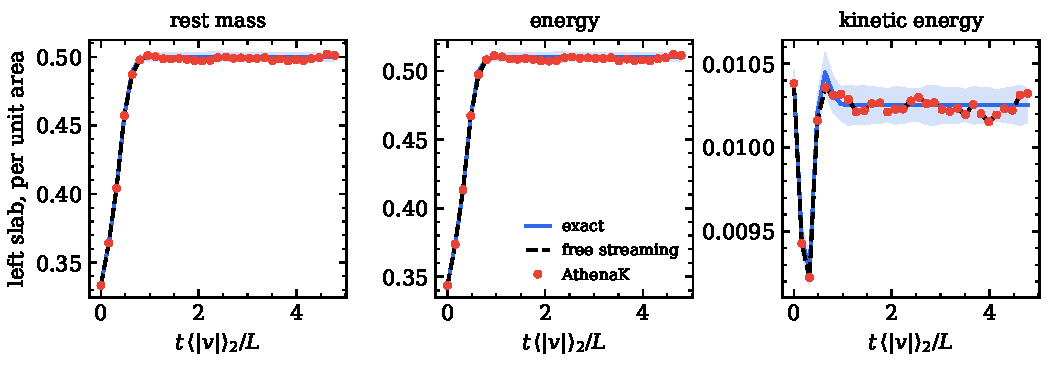
\includegraphics[width=\textwidth]{fig_box_step.pdf}
\caption{Free streaming between two reservoirs in a periodic Minkowski box ($\theta=0.02$ and $0.01$ at equal pressure). Rest mass, energy and kinetic energy in the left slab per unit transverse area against time in units of the box crossing time of the cold gas: the code (dots), straight-line streaming of the same particles (dashed), and the exact ensemble curve with two standard deviations of the sampling noise (blue).}
\label{fig:box}
\end{figure*}

\subsection{The collision operator in the box}\label{sec:t-operator}

Each test of the operator compares a run with an answer fixed before the run (Table~\ref{tab:ledger3}). A replay of one collision step from the code's dump, with the pairings, acceptances and scattering directions rebuilt from the counter-based random numbers, reproduces every collided particle to rounding. The energy and momentum of the whole gas change in a step by a few units of roundoff of their sums, far below the bound of the test [Fig.~\ref{fig:box_summary}(b)]. The number of collisions follows the M\o ller-averaged rate within the sampling noise from cold to ultrarelativistic temperatures, with one sub-step and with sub-cycling of large pair probabilities [Fig.~\ref{fig:box_summary}(a)]. Two gases at different temperatures relax to one Maxwell--J\"uttner distribution at the rate of the reference while the entropy grows monotonically; a gas of unequal macroparticle masses reaches a common temperature; and a run gives byte-identical particles for any division of the mesh and across restarts.

The option that conserves the pair energy at each particle's metric changes nothing in a flat box: it accepts exactly the same collisions as the default in every step, and the momenta differ in the last bits [Fig.~\ref{fig:box_summary}(a,b), open circles]. In the King model at the collisionless threshold the default convention raises the energy measured at the particles' own metric by a small positive amount per collision, because the metric varies across a collision cell; with the option the canonical energy stays constant to rounding (Table~\ref{tab:ledger3}). Production runs in a gravitational field use the option.

In a static curved metric with constant lapse $\alpha_0$ and conformal factor $\psi_0$, proper time runs at $\alpha_0$ and proper volume grows by $\psi_0^6$, so the rate per unit coordinate time and volume must be $\alpha_0\psi_0^6$ times that of a flat twin holding the same particles at their proper positions. Each curved run takes exactly the collisions of its twin in every step, which gives the factor $\alpha_0\psi_0^6$ to rounding, and both agree with the analytic rate within the sampling noise [Fig.~\ref{fig:box_summary}(c)].

\begin{figure*}
\centering
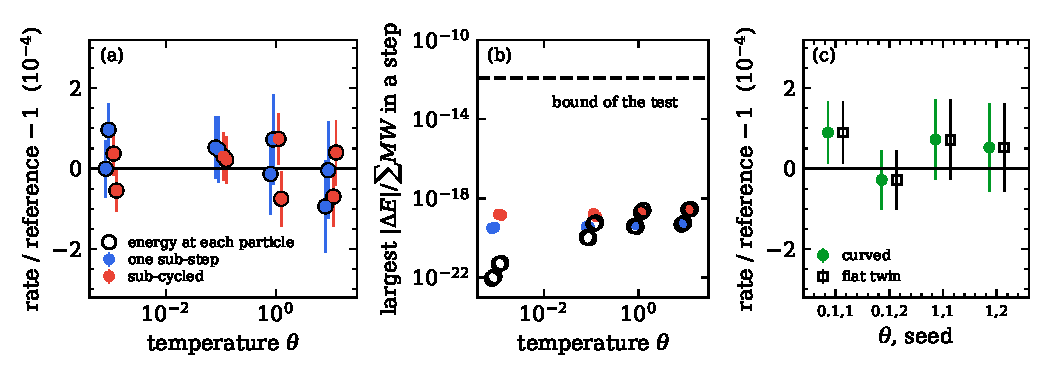
\includegraphics[width=\textwidth]{fig_box_summary.pdf}
\caption{The collision operator in a periodic box. (a) Summed pair probability per step over the M\o ller-averaged rate, minus one, with two standard errors, for one sub-step (blue) and sub-cycling (red); filled: energy at the cell centre, open: at each particle. (b) Largest change of the gas energy in a step over its sum, and the bound of the test. (c) The rate in a static metric with $\alpha_0=0.8$, $\psi_0=1.1$ and in its flat twin.}
\label{fig:box_summary}
\end{figure*}

\subsection{Heat conduction}\label{sec:t-heat}

Conduction drives the gravothermal collapse, so the operator must carry heat at the rate kinetic theory predicts, at both ends of the mean free path. At a long mean free path a temperature step between two slabs streams freely, and the code follows the exact collisionless curve within the sampling noise (Table~\ref{tab:ledger3}). A mode with a wavelength far shorter than the mean free path does the same at all three temperatures tested.

At a short mean free path the step relaxes by conduction. The reference is a one-dimensional gas at uniform pressure with Eckart's heat flux and the conductivity $\kappa=f\kappa_1(T)$, where $\kappa_1$ is the first Chapman--Enskog conductivity of hard spheres and $f$ a free factor; the reference conserves the energy of the box and keeps its volume. Fitted to the rest mass of the initially hot half, $f$ lies within a few hundredths of unity for both seeds [Fig.~\ref{fig:heat}(a,b)]. The residual oscillates with the period of a sound wave crossing the box, which the isobaric reference omits, and the seeds differ by their sampling noise, so this test fixes the conductivity to a few hundredths.

The decay of an isobaric entropy mode measures it more sharply. The rate of the mode at three wavelengths gives $\kappa/\kappa_1$, and its extrapolation to long wavelength lies close to unity, inside the interval the test allows [Fig.~\ref{fig:heat}(c), Table~\ref{tab:ledger3}]. The number-density mode alone carries the sound waves that the initial transient launches and overestimates the conductivity, increasingly at short wavelength; the entropy combination of density and energy removes them. The operator therefore has the Chapman--Enskog conductivity. For the gravothermal fluid models this selects the conduction coefficient $25\sqrt{\pi}/32$ \cite{Koda:2011sidm,Gurian:2025sidm}, which a kinetic code has also reproduced \cite{Gurian:2025sidm}, over the smaller $25\pi/(32\sqrt6)$ of Ref.~\cite{Balberg:2002gt} (Table~\ref{tab:ledger2}). Without sub-cycling the rate stays exact as long as no pair probability exceeds one (Table~\ref{tab:ledger3}).

Hot cores conduct with relativistic particles, where the first Chapman--Enskog approximation loses accuracy. Larger samples on graphics cards add seeds at the cold temperature and extend the mode test to a mildly and a fully relativistic gas [Fig.~\ref{fig:heat}(d)]. With all seeds the cold conductivity stays inside the interval of the test. At the two relativistic temperatures the operator follows the relativistic Chapman--Enskog conductivity at fourth order in the Sonine expansion within its standard error, while the first order lies far below it at the highest temperature; the cold value lies slightly below the fourth order. The relativistic reference was computed independently of the code by a check of this stage, and the comparison was made after the runs. Halving the time step, the cap on the pair probability or the collision cell changes the conductivity by less than the criterion of the convergence test; the conductivity grows with the cell size, a trend that one seed resolves and whose form is open (Table~\ref{tab:ledger3}).

\begin{figure*}
\centering
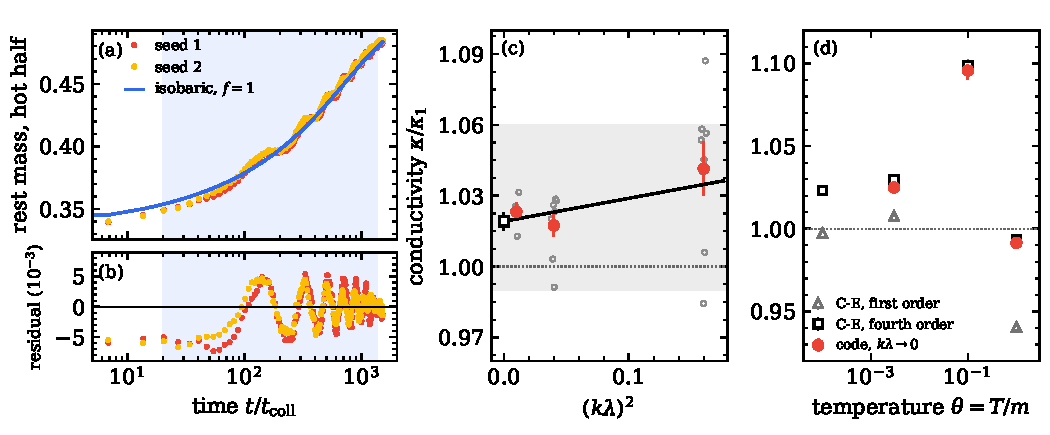
\includegraphics[width=\textwidth]{fig_heat.pdf}
\caption{Heat conduction. (a) Rest mass of the initially hot half of a box with a temperature step ($\theta=0.02$ and $0.01$, $\lambda/L=0.01$) against time in collision times, two seeds, and the isobaric reference with $\kappa_1$; shaded: fit window. (b) Code minus the reference with the fitted $f$. (c) $\kappa/\kappa_1$ from the entropy mode ($\theta=0.003$): seeds (open), their mean (red), extrapolation (line, square); grey band: pass interval. (d) The extrapolated $\kappa/\kappa_1$ from all seeds against temperature, with the relativistic Chapman--Enskog values at first and fourth order.}
\label{fig:heat}
\end{figure*}

\subsection{Initial data in the code}\label{sec:t-id}

The code reads the King threshold model, its metric table and its particle file, and starts the evolution: the particle count and the total rest mass equal those of the model to rounding, and the Hamiltonian-constraint norm is close to that of an earlier monoenergetic set-up. The momentum-constraint norm is larger than in that set-up, and its cause is open (Sec.~\ref{sec:plan}). The code also reads the thermal core at its binding-energy maximum at the larger particle number; the central lapse on the mesh lies slightly above that of the model (Table~\ref{tab:ledger4}).

\subsection{First collisional King clusters}\label{sec:t-clusters}

As a first look at collisions in a relativistic cluster, the two King models CC1, at the collisionless binding-energy maximum, and CC2, slightly less compact and on the stable side of the fluid onset (Fig.~\ref{fig:onsets}), were evolved on a static mesh with collisions at $\Kn_c=10$ and $1$ and without them. These are scouting runs: one seed each, the default energy convention of the operator, and a mesh coarser than the scan will use (Table~\ref{tab:ledger4}).

Both collisionless controls keep every particle bound. With collisions the central lapse of every run falls below that of its control from the start, the sooner the shorter the mean free path, and every collisional run collapses within the evolved time [Fig.~\ref{fig:cluster}(a)]. The energy that the default convention adds at the particles' metric is a small fraction of the binding-energy difference between the two models by the time the lapse has clearly dropped, so the contraction begins without its help; later it grows with the depth of the potential and becomes comparable to that difference (Table~\ref{tab:ledger4}). The four runs collapse after different numbers of collisions per particle and at different times. The pattern fits a gravothermal picture in which collisions carry heat out of the King core, whose velocity dispersion falls outward, and the core contracts across the relativistic threshold; these runs leave that picture a hypothesis.

What the runs establish is that collisions make the core contract relative to its collisionless twin. Three limits keep them from fixing the collisional threshold. The controls drift outward on this mesh by more than CC2 lies from the fluid onset and more than the two models differ [Fig.~\ref{fig:cluster}(b)], so the mesh holds the equilibrium less precisely than the stability margin requires and the collapse of CC2 may be numerical. With one seed per run the scatter of the collapse times between seeds is unmeasured. The static mesh loses the black hole after the collapse, so the rest mass removed by excision is a proxy for the collapsed mass. The decisive runs repeat the pair with the pair energy at each particle's metric and further seeds, refine the mesh, and add a King model on the stable side by more than the drift.

The first of these runs sharpen the limits (Table~\ref{tab:ledger4}). The collapse time of CC1 at $\Kn_c=10$ scatters between seeds far more than that of CC2, as befits a model at its threshold, and the energy convention shifts both within that scatter. On cells of half the size the outward drift of the CC2 control shrinks to a fraction of its value, so the drift is mostly numerical. A King model far on the stable side of both onsets collapses at $\Kn_c=1$ and contracts without collapse at $\Kn_c=10$ within the evolved time, so a collisional collapse needs no proximity to the relativistic onset. These runs leave the collisional threshold and the collapsed mass open, and enter the next version with their figures.

\begin{figure*}
\centering
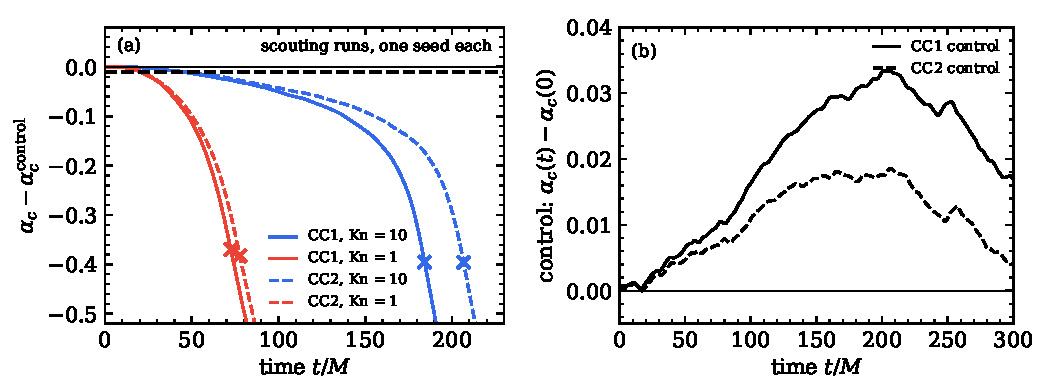
\includegraphics[width=\textwidth]{fig_cluster.pdf}
\caption{First collisional King clusters (scouting, one seed each). (a) Central lapse of each collisional run minus that of its collisionless control, CC1 (solid) and CC2 (dashed) at $\Kn_c=10$ and $1$, up to the first excision; crosses: smallest lapse on the mesh below $0.3$; dashed line: a drop of $0.01$. (b) Central lapse of the two controls minus its first value.}
\label{fig:cluster}
\end{figure*}

\section{Toward the capability gate: the collisionless threshold}\label{sec:g2}

A King cluster beyond the turning point of its equilibrium sequence collapses once its radial mode is kicked inward; a cluster before the turning point oscillates and keeps its particles bound. The code locates the collisionless threshold by evolving two King models that sit on either side of the turning point, each kicked inward by the same small fraction of its radial velocity, beside unkicked controls that must hold their equilibrium over the whole evolved time. A run counts as collapsed when the smallest lapse on the mesh falls below a fixed marker value. None of these runs carries an apparent-horizon finder, so every collapse time below is a lapse marker. The models, meshes and markers are listed in Table~\ref{tab:ledgerG2}.

\subsection{Particle noise sets the life of a control}\label{sec:g2-noise}

The controls decide which particle number can locate the threshold. At the intermediate particle number of the scan all three controls collapse late in the evolved time, in an order unrelated to their compactness, and a kicked stable model outlives its own control. The control of the threshold model collapses earlier with ten times fewer particles and holds its equilibrium with ten times more, where it pulsates slowly with no secular contraction. Across the three particle numbers the floor of the Hamiltonian constraint falls as the inverse particle number, the signature of the deposit noise of the particles. The collapse time of a control grows with the particle number, though much more slowly than the particle number itself. Particle noise therefore drives the control collapse, and the threshold is read at the largest particle number.

\subsection{The bracket at a million particles}\label{sec:g2-bracket}

At the largest particle number on the standard mesh the two kicked models part ways. The more compact model collapses within the first half of the evolved time; the less compact one oscillates inside a narrow band around the control of the threshold model to the end. The two models straddle the turning point of the King family (Table~\ref{tab:parameters}), so the code places the collisionless threshold between them, as the turning-point criterion of Ref.~\cite{Gunther:2020ev} requires. The same pair has the same fates at ten times fewer particles, where the unstable member collapses somewhat earlier. Each member has one seed, and the bracket rests on one mesh and one gauge; the members on the finer mesh and with weaker shift damping are the last runs of the capability gate.

\subsection{Collisional collapse on three meshes and in two gauges}\label{sec:g2-collisional}

With collisions at $\Kn_c=10$ the cluster CC2 collapses on all three meshes. The coarsest mesh lies outside the asymptotic range: its collapse comes much later than on the two finer meshes, which differ by a few times the scatter between runs on the standard mesh that change only the collision seed, the collision cell or the shift damping. Halving the shift damping moves the collapse time by less than that scatter and leaves the collision rate unchanged; after the collapse, the run with weaker damping ends in non-finite fields on the static mesh. The collisions conserve energy to rounding in the curved spacetime on both finer meshes and in both gauges (Table~\ref{tab:ledgerG2}).

\section{Plan and open questions}\label{sec:plan}

Figure~\ref{fig:timeline} shows the gates of the track. The scoping gate is complete with this note. For the baseline gate the spherical baseline, the box tests of the operator, the conduction at both ends of the mean free path and the fluid anchor are in this note, and an independent recomputation of the baseline numbers from the run outputs has been made. The capability gate locates the collisionless thresholds of the three families with three-way convergence and closes the conservation budgets of the collisions in curved spacetime. The science gate gives the collapsed mass fraction against the Knudsen number for thermal cores on both sides of the collisionless threshold.

Five items stand between the gates. (i) The growth rate of the radial mode: the fit recovers the rates of synthetic signals, and the analysis recovers the published outcomes of the monoenergetic runs of Ref.~\cite{Wu:2026nrpic}; on the unstable runs of that reference the logarithm of the perturbation is concave from the start, so a growth rate holds only over a stated interval, and the threshold scan relies on collapse times and on the contraction against a control (Table~\ref{tab:ledger4}). (ii) The rest of the decisive cluster runs of Sec.~\ref{sec:t-clusters}: the threshold model on the finer mesh, the collision cell size, and at least three seeds per model near the threshold. (iii) Collisions on refined meshes and an energy diagnostic of the whole spacetime in the code, so that runs follow the black hole and close their energy budget. (iv) The cost of a collision, which fixes how small a Knudsen number the computing time reaches; the particle number grows as $\Kn^{-3}$ and the collision term is stiff at small $\Kn$. (v) The momentum-constraint excess of Sec.~\ref{sec:t-id}. The capability and science gates need more computing time than the current allotment.

\begin{figure*}
\centering
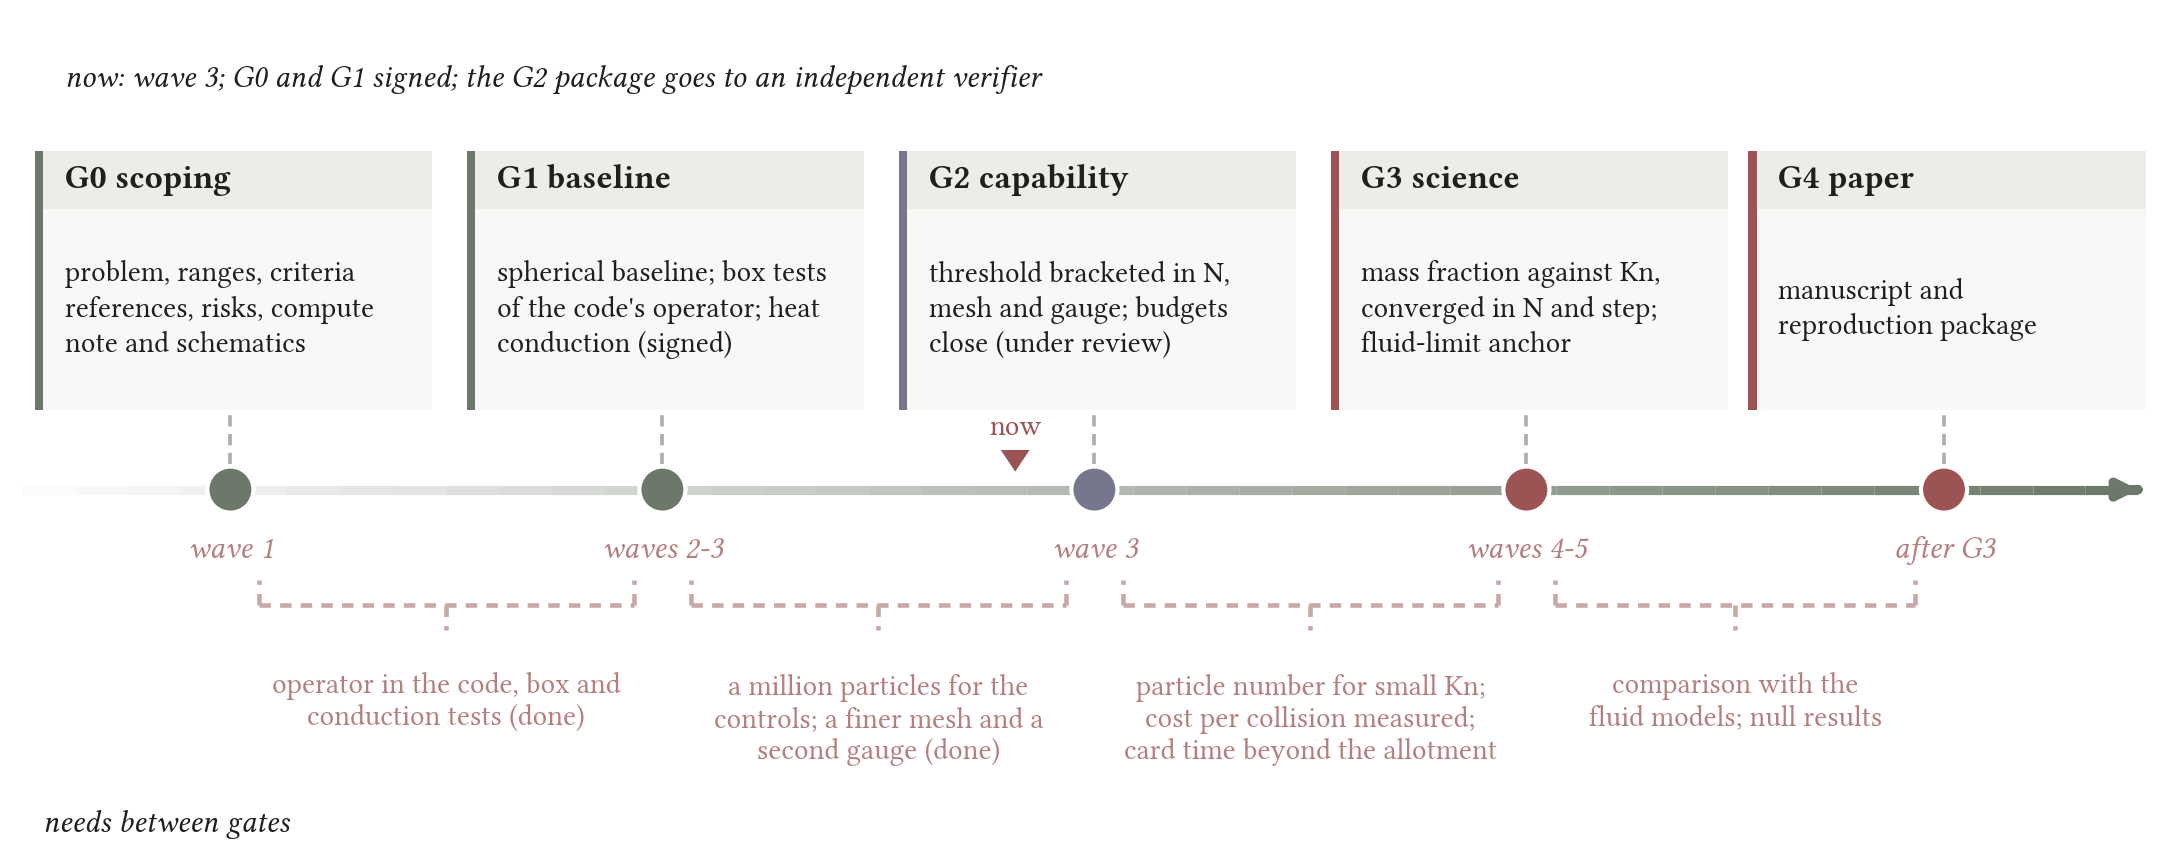
\includegraphics[width=0.92\textwidth]{schem_timeline.png}
\caption{Stage timeline. Each gate (circle) with its evidence (box above) and what the step to it needs (below); the marker shows the present state.}
\label{fig:timeline}
\end{figure*}

\section{Summary}\label{sec:summary}

Real relativistic cores of self-interacting dark matter are collision-dominated by a margin of twelve to twenty orders of magnitude, so a particle calculation reaches them only through a bridge: a scan in the Knudsen number from collisionless clusters to the fluid limit, with the exact pulsation onset of the same equilibrium as its anchor. With the adiabatic index of a collision-dominated relativistic gas that anchor sits just on the stable side of the collisionless turning point, so collisions can move the threshold only within a narrow band, and resolving that band sets the precision the cluster runs need. The collision operator that drives the scan conserves each pair's four-momentum, counts collisions with a Lorentz-invariant speed, keeps the relativistic rate in curved spacetime, and conducts heat as kinetic theory predicts. With collisions, King clusters contract against their collisionless twins and collapse; whether a cluster on the stable side of the fluid onset collapses too waits for a mesh that holds the equilibrium within the stability margin.

\begin{acknowledgments}
This note, its figures and the calculations behind it were produced by large-language-model agents (Claude, Anthropic) working in the program's repository under human direction; the agents' records of predictions and outcomes are kept with the runs.
\end{acknowledgments}

\appendix

\section{Parameters of the models}\label{app:parameters}

Table~\ref{tab:parameters} lists the equilibrium models at the instability criteria of Sec.~\ref{sec:t-sequences}, in units of the ADM mass.

% generated by scripts/ledger.py from registered run outputs; do not edit
\begin{table}
\caption{The equilibrium models at the instability criteria. $Z(0)$ or $z_c$: central redshift; $\epsilon$: binding-energy fraction; $R$: areal radius; $M$: ADM mass.}
\label{tab:parameters}
\begin{ruledtabular}
\begin{tabular}{lcccc}
Model & parameter & $Z(0)$ & $\epsilon$ & $R/M$ \\
\hline
thermal core, $\epsilon$ maximum & $w_0=3.1652$ & 0.5404 & 0.03518 & 20.44 \\
thermal core, onset $1+p/u$ & $w_0=3.5871$ & 0.6348 & 0.03467 & 22.18 \\
thermal core, onset $5/3$ & $w_0=4.1603$ & 0.7792 & 0.03248 & 27.13 \\
thermal core, trial & $w_0=4.0511$ & 0.7500 & 0.03302 & 25.87 \\
King threshold & $y_0=0.33403$ & 0.5119 & 0.03559 & 13.63 \\
monoenergetic threshold & $y_c=0.67961$ & 0.4553 & 0.03606 & 6.55 \\
\end{tabular}
\end{ruledtabular}
\end{table}


\section{Numerical ledger and data flow}\label{app:ledger}

Tables~\ref{tab:ledger}--\ref{tab:ledger4} give every number behind this note with the registered run that produced it; the inputs of each figure and table were checked against the checksums their runs recorded, and Fig.~\ref{fig:dataflow} shows the path from the initial data to the figures. The figures and tables of this version were made in run \texttt{C-20261127-084828-b6ca5ce\unskip}; the scoping-stage numbers equal those of runs C-20261115-171741-0e0da67 and C-20261115-170415-385069e. Numbers quoted from the literature, with their locators in the arXiv sources of the knowledge base: the black hole of the fluid calculation, about $200\,M_\odot$ at $580\,t_0$ for a fiducial halo with $\sigma/m=5\,$cm$^2$/g, a collapse fraction of about $3\times10^{-8}$ (Ref.~\cite{Gu:2026sidm}, \texttt{SIDM\_MS.tex} lines 68, 384, 481); the seed of the J1205-0000 benchmark, $1.9\times10^{9}\,M_\odot$ (Ref.~\cite{Feng:2021instab}, \texttt{main.tex} line 349); the printed King thresholds $y_{\max}=0.334$ and $y_{\rm zero}=0.784$ (Ref.~\cite{Gunther:2020ev}, \texttt{paper.tex} line 953); the printed binding-energy maximum $0.0352$ at $Z(0)=0.548$ for $b=0.1$ (Ref.~\cite{Feng:2021instab}, \texttt{main.tex} line 280); its trial-function onset $Z(0)=0.750$ and its remark that the onset is insensitive to the trial function (\texttt{main.tex} lines 274 and 220), and the exact mode with the same index recomputed independently in run C-20261121-080313-84094f1; the agreement of $N$-body and conducting fluid for $\Kn\ge1$ (Ref.~\cite{Koda:2011sidm}, \texttt{sidm1.tex} lines 1482--1491); the conduction coefficient $b=25\sqrt{\pi}/32$ (Ref.~\cite{Koda:2011sidm}, \texttt{sidm1.tex} lines 409--412; Ref.~\cite{Gurian:2025sidm}, \texttt{sidm.tex} line 163) and $25\pi/(32\sqrt6)$ (Ref.~\cite{Balberg:2002gt}, \texttt{SIDMGT\_Xiv2.tex} line 394); the kinetic code of Ref.~\cite{Gurian:2025sidm} reproduces the Chapman--Enskog conductivity to within two percent (\texttt{sidm.tex} line 94). The second driver of the kernel test is core's run core-20261115-132556-a7dc8ab (the same largest errors to all printed digits). Of 23 numbers quoted in the stage documents of the track, 20 agree with the run outputs and 3 differ\unskip: the stage documents bound the deviation from the printed table of Ref.~\cite{Feng:2021instab} by a value that three columns exceed at one row, give the fastest gravothermal phase as at least $10^5$ dynamical times where the run gives a lower bound of $8.5\times10^4$, and quote radius ranges of the thermal-core models that hold for a narrower range of central redshift than stated. The conduction runs on graphics cards are runs C-20261119-150335-73fd40f and C-20261119-150347-e100007, reduced in runs C-20261120-221630-fd17a2d and C-20261120-222329-3a77ad6.

% generated by scripts/ledger.py from registered run outputs; do not edit
\begin{table*}
\caption{Numerical ledger of the scoping stage. Every number of this note with the registered run that produced it.}
\label{tab:ledger}
\begin{ruledtabular}
\footnotesize
\begin{tabular}{p{0.41\textwidth}p{0.27\textwidth}p{0.23\textwidth}}
Quantity & Value & Run \\
\hline
\multicolumn{3}{l}{\emph{Spherical baseline}} \\
rows of the two printed tables of Ref.~\cite{Feng:2021instab} compared & 56; 14 & \texttt{\scriptsize C-sidm-20261115-120722-38ab057} \\
largest relative difference, columns other than the radius (column, line) & $2.43\times10^{-4}$ (B, 503) & \texttt{\scriptsize C-sidm-20261115-120722-38ab057} \\
largest relative difference of the radius (printed to three digits) & $2.45\times10^{-3}$ & \texttt{\scriptsize C-sidm-20261115-120722-38ab057} \\
printed values off by more than ten percent (line, column) & 491 C, 493 p0, 516 C & \texttt{\scriptsize C-sidm-20261115-120722-38ab057} \\
largest relative difference of the root $w_0$ of the second table & $1.10\times10^{-4}$ & \texttt{\scriptsize C-sidm-20261115-120722-38ab057} \\
$b=0.1$: binding-energy maximum, $w_0$; $Z(0)$; $\epsilon$; $v(0)$ & 3.16524; 0.54041; 0.035179; 0.5035 & \texttt{\scriptsize C-sidm-20261115-120722-38ab057} \\
$b=0.1$: pulsation onset, $\Gamma=1+p/u$, $w_0$; $Z(0)$; $\epsilon$; $v(0)$ & 3.5871; 0.63482; 0.034674; 0.5342 & \texttt{\scriptsize C-sidm-20261115-120722-38ab057} \\
$b=0.1$: pulsation onset with $\Gamma=5/3$, $Z(0)$; trial criterion $w_0$, $Z(0)$ & 0.77924; 4.05115, 0.75001 & \texttt{\scriptsize C-sidm-20261115-120722-38ab057} \\
$b=0.2, 0.3, 0.5$: $Z(0)$ of the binding-energy maximum; of the onset ($1+p/u$) & 0.5225, 0.5176, 0.5142; 0.5923, 0.5843, 0.579 & \texttt{\scriptsize C-sidm-20261115-120722-38ab057} \\
pulsation zero against the mass maximum, $\Gamma=2$ polytropes, three resolutions & $2.7\times10^{-8}$, $1.5\times10^{-8}$, $2.5\times10^{-8}$ & \texttt{\scriptsize C-sidm-20261115-121524-5cebcf5} \\
two independent thermal-core solvers, $b=0.1$ grid: largest relative difference in $\epsilon$; absolute in $Z(0)$ & $2.0\times10^{-8}$; $2.0\times10^{-9}$ & \texttt{\scriptsize C-sidm-20261115-131130-3077a99} \\
lowest $\omega_0^2$ at the onset, two resolutions & $-2.3\times10^{-6}$, $-4.5\times10^{-6}$ & \texttt{\scriptsize C-sidm-20261115-131130-3077a99} \\
King: binding-energy maximum $y_0$; $z_c$; fraction; first zero $y_0$ (printed 0.334, 0.784, Ref.~\cite{Gunther:2020ev}) & 0.334032; 0.51191; 0.035589; 0.78452 & \texttt{\scriptsize C-sidm-20261115-115348-eb8b752} \\
King: two solvers, largest relative difference of the fraction; of $z_c$ & $3.5\times10^{-8}$; $6.5\times10^{-10}$ & \texttt{\scriptsize C-sidm-20261115-131130-3077a99} \\
monoenergetic: maximum $y_c$; $z_c$; fraction; $R/M$ & 0.67961; 0.45529; 0.036058; 6.552 & \texttt{\scriptsize C-sidm-20261115-115344-eb8b752} \\
monoenergetic: 5 models of Ref.~\cite{Wu:2026nrpic}, largest difference of $z_c$; relative of $R/M$ & $4.3\times10^{-4}$; $9.3\times10^{-6}$ & \texttt{\scriptsize C-sidm-20261115-115344-eb8b752} \\
thermal-core models $Z(0)=0.40$--$0.80$: $R/M$; $r_{\rm core}/M$; central lapse & 19.8--28.1; 1.27--2.56; 0.556--0.714 & \texttt{\scriptsize C-sidm-20261115-121748-4e8d6b5} \\
\multicolumn{3}{l}{\emph{Particle models and Knudsen number}} \\
particle models; particles each; offline checks passed of total & 13; 10000; 243 of 243 & \texttt{\scriptsize C-sidm-20261115-121626-e99907d} \\
$K=\tilde\sigma\,{\rm Kn}_c$: King threshold model; range over the 13 models & 168.895; 154.3--206.5 & \texttt{\scriptsize C-sidm-20261115-131130-3077a99} \\
$K$ with the energy density in $H$; ratio of the transport mean free path to $\lambda$ & 198.64; 0.766--0.797 & \texttt{\scriptsize C-sidm-20261115-131130-3077a99} \\
$\sigma/m$ in cm$^2$/g for $\tilde\sigma=1$ and $M=M_\odot$ & $1.0966\times10^{-23}$ & \texttt{\scriptsize C-sidm-20261115-131130-3077a99} \\
${\rm Kn}_c$ at $\sigma/m=5\,$cm$^2$/g, $M=200\,M_\odot$; $1.9\times10^9\,M_\odot$ (13 models) & $6.8\times10^{-20}$--$9.1\times10^{-20}$; $6.4\times10^{-13}$--$8.6\times10^{-13}$ & \texttt{\scriptsize C-sidm-20261115-131130-3077a99} \\
the same with the energy density in $H$, six candidate models & $4.5\times10^{-20}$--$1.8\times10^{-19}$; $4.3\times10^{-13}$--$1.7\times10^{-12}$ & \texttt{\scriptsize C-sidm-20261115-115400-eb8b752} \\
King threshold model: $H_c/M$; central particle spacing at $10^4$ particles & 1.4359; 0.293 & \texttt{\scriptsize C-sidm-20261115-122915-cdc395c} \\
code reads the King threshold files: particles; rest mass against the model; Hamiltonian; momentum constraint norm over the reference & 10000; $3.0\times10^{-14}$; 0.932; 1.419 & \texttt{\scriptsize C-sidm-20261115-125308-54870b9} \\
\end{tabular}
\end{ruledtabular}
\end{table*}
\begin{table*}
\caption{Numerical ledger of the scoping stage, continued.}
\label{tab:ledger2}
\begin{ruledtabular}
\footnotesize
\begin{tabular}{p{0.41\textwidth}p{0.27\textwidth}p{0.23\textwidth}}
Quantity & Value & Run \\
\hline
\multicolumn{3}{l}{\emph{Collision operator: references and kernel test}} \\
closed-form mean M\o ller speed against quadrature: largest relative difference ($\theta$); at $\theta=100$ & $5.17\times10^{-7}$ (0.001); $2.5\times10^{-14}$ & \texttt{\scriptsize C-sidm-20261115-131130-3077a99} \\
Monte Carlo pair average of the rate, 11 temperatures, deviation in standard errors & -1.30 to +0.98 & \texttt{\scriptsize C-sidm-20261115-120703-9b3e868} \\
two-temperature relaxation rate, Monte Carlo over quadrature at $\theta=10^{-3}, 0.1, 1, 10$ & 1.0048$\pm$0.0029, 0.9990$\pm$0.0025, 1.0014$\pm$0.0022, 1.0029$\pm$0.0022 & \texttt{\scriptsize C-sidm-20261115-120703-9b3e868} \\
relaxation rate over its non-relativistic form at $\theta=0.001, 0.053, 2.81, 100$ & 0.9954, 0.8129, 0.1622, 0.02714 & \texttt{\scriptsize C-sidm-20261115-120703-9b3e868} \\
pair kinematics: largest error against the 60-digit oracle; momentum; energy residual (units of $\varepsilon$) & $9.7\times10^{-16}$; 0.72; 2.58 & \texttt{\scriptsize C-sidm-20261115-120703-9b3e868} \\
conductivity coefficient $\kappa_1\sigma/\sqrt\theta$; ratio to the constant of Ref.~\cite{Balberg:2002gt} & 2.0771; 1.382 & \texttt{\scriptsize C-sidm-20261115-120703-9b3e868} \\
entropy gap per particle at $\theta_2=10^{-3}$; $\theta_2=1$ & 0.0448; 0.1232 & \texttt{\scriptsize C-sidm-20261115-120703-9b3e868} \\
kernel test on the code: cases (skipped); largest velocity error; four-momentum residual ($\varepsilon$); failures & 208 (1); $3.22\times10^{-16}$; 1.32; 0 & \texttt{\scriptsize C-sidm-20261115-132624-13a77db} \\
\multicolumn{3}{l}{\emph{Minkowski box in the code}} \\
free streaming in the box: particles; $\theta_1$; $\theta_2$ (measured); snapshots & 100000; 0.02026; 0.01000; 31 & \texttt{\scriptsize C-sidm-20261115-121302-313d399} \\
largest position error over the box length; code against free streaming of the sample (relative) & $1.81\times10^{-12}$; 0 & \texttt{\scriptsize C-sidm-20261115-121302-313d399} \\
deviation from the ensemble in noise units, largest; rms (rest mass, energy, kinetic energy) & 1.85, 1.85, 1.85; 1.01, 1.01, 0.82 & \texttt{\scriptsize C-sidm-20261115-121302-313d399} \\
planned rate test: expected collisions per step at $\theta=0.001, 0.1, 1.0, 10.0$ & 1472, 1993, 2744, 2778 & \texttt{\scriptsize C-20261115-165028-a559ab8} \\
\multicolumn{3}{l}{\emph{Time scales and costs}} \\
fluid model, collapsing core: $t_0/t_{\rm dyn}$; fastest phase over $t_{\rm dyn}$; ${\rm Kn}$ of the core (lower bounds) & $8.52\times10^{5}$; $8.52\times10^{4}$; $1.94\times10^{-6}$ & \texttt{\scriptsize C-sidm-20261115-121412-d463e1a} \\
cost of existing cluster runs at $10^4$ particles, s per $M$: static $M/2$; static $M/4$; adaptive & 1.67; 3.28--3.71; 14.2--17.5 & \texttt{\scriptsize C-sidm-20261115-115400-eb8b752} \\
\end{tabular}
\end{ruledtabular}
\end{table*}
\begin{table*}
\caption{Numerical ledger of the baseline stage: the collision operator.}
\label{tab:ledger3}
\begin{ruledtabular}
\footnotesize
\begin{tabular}{p{0.41\textwidth}p{0.27\textwidth}p{0.23\textwidth}}
Quantity & Value & Run \\
\hline
\multicolumn{3}{l}{\emph{Collision operator in the box: released operator and energy at each particle's metric}} \\
replay of one collision step (released): dumps reproduced & 6 of 6 & \texttt{\scriptsize C-20261115-170155-13ff01f} \\
replay of one collision step (energy at each particle): dumps reproduced & 6 of 6 & \texttt{\scriptsize C-20261119-141711-7db7a6a} \\
rate test, 16 runs (released): summed pair probability over the M\o ller-averaged rate; $z$; largest energy change per step over its bound & 0.999906--1.000096; -2.20 to +2.92; $1.08\times10^{-7}$ & \texttt{\scriptsize C-20261115-165500-c67e036} \\
rate test, 16 runs (energy at each particle): summed pair probability over the M\o ller-averaged rate; $z$; largest energy change per step over its bound & 0.999906--1.000096; -2.20 to +2.92; $1.05\times10^{-7}$ & \texttt{\scriptsize C-20261119-141806-af19c1c} \\
the two operators in the flat box: tested pairs and collisions identical in every step; largest relative difference of the rate ratio & yes; $4.4\times10^{-16}$ & \texttt{\scriptsize C-20261115-165500-c67e036} \texttt{\scriptsize C-20261119-141806-af19c1c} \\
reproducibility (released): runs byte-identical to one MeshBlock; collisions & 5 of 5 (other seed differs); 385554 & \texttt{\scriptsize C-20261115-165902-f9b1c8f} \\
reproducibility (energy at each particle): runs byte-identical to one MeshBlock; collisions & 5 of 5 (other seed differs); 385554 & \texttt{\scriptsize C-20261119-143041-f94e350} \\
released operator: relaxation, initial relaxation rate, entropy (four runs each); unequal macroparticle masses (eight seeds; Kolmogorov--Smirnov test against the temperature of each mass class) & pass, pass, pass; pass & \texttt{\scriptsize C-20261115-170539-28432c3} \texttt{\scriptsize C-20261115-170814-8a54b43} \\
static curved metric (lapse 0.8, conformal factor 1.1): rate per coordinate time and volume over the flat twin; $\alpha_0\psi_0^6$; analytic rate ratio; largest $|z|$ & 1.4172488--1.4172488; 1.4172488; 0.999972--1.000090; 2.35 & \texttt{\scriptsize C-20261119-145925-dbcfb9c} \\
King threshold model, first step: energy change per collision over its sum, released operator (cell sums, Kn$_c=0.01$); energy at each particle & 8.00e-11 $\pm$ 3.4e-11; 1.7e-21--2.0e-21 & \texttt{\scriptsize C-20261119-141431-a351ac7} \\
\multicolumn{3}{l}{\emph{Heat conduction}} \\
step at $\lambda/L=1000$, two seeds: rms deviation from the collisionless curve in noise units (rest mass, energy, kinetic energy); initial slopes over the exact & 1.20, 1.20, 1.11; 0.86, 0.87, 1.04; 1.001, 0.978 & \texttt{\scriptsize C-20261119-152744-2bba6de} \\
step at $\lambda/L=0.01$: conductivity factor $f$ of the two seeds; late window; mean and standard error; literal statistic & 1.029, 1.063; 1.036, 1.066; 1.046 $\pm$ 0.017; 0.994, 1.027 & \texttt{\scriptsize C-20261119-160003-287b389} \\
isobaric mode, $\theta=0.003$: $\kappa/\kappa_1$ from the entropy mode at $k\lambda=0.1, 0.2, 0.4$ (seeds) & 1.0232 $\pm$ 0.0039 (4); 1.0174 $\pm$ 0.0047 (8); 1.0414 $\pm$ 0.0114 (8) & \texttt{\scriptsize C-20261119-161930-acd257b} \\
the same from the number-density mode alone (biased by sound waves; fit window of the track's analysis) & 1.052, 1.111, 1.448 & \texttt{\scriptsize C-20261119-161930-acd257b} \\
extrapolated to $k\lambda\to0$: $\kappa/\kappa_1$; pass interval & 1.0192 $\pm$ 0.0038; [0.99, 1.06] & \texttt{\scriptsize C-20261119-161930-acd257b} \\
collisionless mode ($k\lambda=100$) at $\theta=0.003, 0.1, 1$: largest $|z|$ against the ensemble & 3.03, 3.08, 2.89 & \texttt{\scriptsize C-20261119-152845-017d186} \\
isobaric mode at $\theta=0.003, 0.1, 1$, all seeds (processors and card, weights proportional to $N$), extrapolated: $\kappa/\kappa_1$ & 1.0250 $\pm$ 0.0025; 1.0957 $\pm$ 0.0051; 0.9914 $\pm$ 0.0035 & \texttt{\scriptsize C-20261120-223203-b38a7d7} \\
relativistic Chapman--Enskog conductivity of hard spheres, fourth order, at the same $\theta$; first order at $\theta=1$ & 1.0296 $\pm$ 0.0010; 1.0988 $\pm$ 0.0015; 0.9933 $\pm$ 0.0010; 0.9407 & \texttt{\scriptsize C-20261120-222423-519f12b} \texttt{\scriptsize C-20261121-030328-e3ffc6d} \\
code minus fourth-order reference, in standard errors of the code (same order) & -1.72, -0.58, -0.51 & \texttt{\scriptsize C-20261121-030328-e3ffc6d} \\
convergence on a graphics card (one seed, $4\times10^6$ particles, $\theta=0.003$, $k\lambda=0.2$): $f$ at three values of the step, largest pair probability, cell size & 1.0169/1.0222/1.0203; 1.0221/1.0222/1.0274; 1.0116/1.0222/1.0403 & \texttt{\scriptsize C-20261120-223321-3d088d4} \\
relative change of $f$ between the two finest values (same order); criterion & -0.0052, -0.0001, -0.0104; below 0.02 in magnitude & \texttt{\scriptsize C-20261120-223321-3d088d4} \\
rate at a largest pair probability of 0.56 without sub-cycling; with sub-cycling & 1.000025 $\pm$ 0.000041; 0.999992 $\pm$ 0.000026 & \texttt{\scriptsize C-20261119-151044-a584069} \\
\end{tabular}
\end{ruledtabular}
\end{table*}
\begin{table*}
\caption{Numerical ledger of the baseline stage: models, onsets and the first collisional clusters.}
\label{tab:ledger4}
\begin{ruledtabular}
\footnotesize
\begin{tabular}{p{0.41\textwidth}p{0.27\textwidth}p{0.23\textwidth}}
Quantity & Value & Run \\
\hline
\multicolumn{3}{l}{\emph{Particle models and onsets}} \\
particle models at $N=10^5$: thermal core; King; offline checks passed (failures: the check's own step error) & 8; 5; 240 of 243 & \texttt{\scriptsize C-20261115-170742-84990ed} \texttt{\scriptsize C-20261115-171137-9e3c807} \\
conversion constant $K$ over these models & 110.46--186.08 & \texttt{\scriptsize C-20261115-193751-d3872ff} \\
code reads the thermal core at its binding-energy maximum: particles; central lapse on the mesh; of the model & 100000; 0.65411; 0.64918 & \texttt{\scriptsize C-20261115-174557-8978b36} \texttt{\scriptsize C-20261115-170742-84990ed} \\
thermal core: $Z(0)$ of the binding-energy maximum; J\"uttner onset (energy-matched temperature; $\theta=p/n$); onset with $\Gamma=1+p/u$ & 0.54041; 0.53306; 0.53170; 0.63482 & \texttt{\scriptsize C-20261115-165315-7b473b8} \\
King: $y_0$ of the binding-energy maximum; J\"uttner onset (central lapse); $\theta=p/n$; $\Gamma=1+p/u$ & 0.334032; 0.32143 (0.6707); 0.32054; 0.37206 & \texttt{\scriptsize C-20261119-151502-cb831a8} \\
central lapse of the cluster-run models CC2 ($y_0=0.314$); CC1 ($y_0=0.33403$) & 0.6762; 0.6614 & \texttt{\scriptsize C-20261115-170742-84990ed} \\
growth-rate fit on synthetic signals, true rates 0.02, 0.05, 0.1 (50 signals each): mean relative bias; rms relative error & -1.6e-05, 0.004; -6.1e-04, 0.005; +6.9e-04, 0.007 & \texttt{\scriptsize C-20261120-222716-9d86ebc} \\
published outcomes of the earlier monoenergetic runs (horizon times and masses, particles left, lapse crossing times, half-swing growth) recovered by the analysis & 18 of 18 & \texttt{\scriptsize C-20261120-222716-9d86ebc} \\
unstable monoenergetic runs ($y_c=0.5$, three samples): local growth rate at the start and the end of the analysed interval ($1/M$); rate over the common interval 17.5--51.75 $M$ & 0.075/0.026; 0.082/0.023; 0.082/0.025; 0.0557, 0.0584, 0.0617 & \texttt{\scriptsize C-20261120-223404-40668db} \\
\multicolumn{3}{l}{\emph{First collisional King clusters (scouting, one seed each)}} \\
central lapse 0.01 below the control (CC1, CC2 at Kn$_c=10$; at 1), $t/M$ & 44.25, 46, 20.25, 21.25 & \texttt{\scriptsize C-20261115-171058-c26cfad} \texttt{\scriptsize C-20261115-171059-4b70228} \texttt{\scriptsize C-20261115-171059-35441e3} \\
smallest lapse below 0.3, $t/M$ (same order) & 184.25, 206.75, 72.5, 77.75 & \texttt{\scriptsize C-20261115-171058-c26cfad} \texttt{\scriptsize C-20261115-171059-4b70228} \texttt{\scriptsize C-20261115-171059-35441e3} \\
controls: largest rise of the central lapse (at $t/M$), CC1; CC2 & 0.0334 (201.5); 0.0185 (206.75) & \texttt{\scriptsize C-20261115-171058-c26cfad} \texttt{\scriptsize C-20261115-171059-4b70228} \\
collisions per particle before the lapse falls below 0.3 (same order) & 2.48, 2.88, 13.44, 15.26 & \texttt{\scriptsize C-20261119-151502-cb831a8} \\
energy injected by the released operator by the 0.01 drop, over the binding-energy margin of CC1 and CC2 ($1.0\times10^{-4}$ $M_0$) (same order) & 0.016, 0.013, 0.117, 0.108 & \texttt{\scriptsize C-20261119-151944-08f3220} \\
\multicolumn{3}{l}{\emph{Follow-up cluster runs (scouting; reported in full in the next version)}} \\
CC1 at Kn$_c=10$: collapse time (interpolated first crossing of 0.3 by the smallest lapse) of three seeds, released operator; standard deviation; two seeds with the energy at each particle & 184.02, 185.29, 178.86; 3.40; 184.93, 185.85 ($M$) & \texttt{\scriptsize C-20261121-075202-1a37fb9} \\
CC2 at Kn$_c=10$, two seeds of each operator: range of the collapse time; standard deviation & 206.26--206.73; 0.21 ($M$) & \texttt{\scriptsize C-20261121-075202-1a37fb9} \\
King model with $y_0=0.26$: collapse time at Kn$_c=1$; at Kn$_c=10$ & 100.46 $M$; none by 300 $M$ & \texttt{\scriptsize C-20261121-075202-1a37fb9} \\
CC2 control on cells of half the size: outward excursion of the central lapse over that on the coarse mesh (cosine amplitude; sine with trend; largest mean over $20M$) & 0.22; 0.25; 0.10 & \texttt{\scriptsize C-20261121-075359-26e3b31} \\
\end{tabular}
\end{ruledtabular}
\end{table*}


\begin{table*}
\caption{Numbers behind Sec.~\ref{sec:g2}, written from the registered analyses named in the last column (one seed per run unless stated). A run collapses when the smallest lapse on the mesh falls below $0.3$; no run carries a horizon finder. Kicks are inward, one percent of the radial velocity. M/8 and M/16: cell size of the core region in units of the ADM mass; the shift damping is $2$ unless stated.}
\label{tab:ledgerG2}
\footnotesize
\begin{ruledtabular}
\begin{tabular}{p{5.6cm}p{3.0cm}p{3.9cm}p{4.2cm}}
Quantity & Runs & Value & Analysis \\
\hline
Control $y_0=0.334032$, M/8: collapse time & $N=10^4$, $10^5$, $10^6$ & $295.78$, $534.81\,M$, none by $600\,M$ & C-20261126-120656-f5c62bb \\
Same: Hamiltonian-constraint floor, $100$--$300\,M$ & $N=10^4$, $10^5$, $10^6$ & $7.68\times10^{-2}$, $7.86\times10^{-3}$, $7.90\times10^{-4}$ & same \\
Controls $y_0=0.344$, $0.324$, $N=10^5$: collapse time & M/8 & $549.26$, $599.99\,M$ & C-20261125-160056-a5b7282 \\
Kicked $y_0=0.344$: collapse time & $N=10^6$, $10^5$ & $252.31$, $229.79\,M$ & C-20261126-121836-c7a76c1 \\
Kicked $y_0=0.324$: central lapse change, $20\,M$ means to $600\,M$ & $N=10^6$ & $-0.0119$ to $+0.0150$, no collapse & same \\
Same & $N=10^5$ & $-0.0248$ to $-0.0024$, no collapse & same \\
CC2, $\Kn_c=10$: collapse time on M/4, M/8, M/16 & collision cell M/4 & $206.64$, $163.41$, $158.42\,M$ & C-20261126-121702-b6b1eda (M/4: mean of earlier seeds) \\
Same on M/8: other collision seed, cells M/8, M/2, shift damping $1$ & one change each & $165.65$, $164.01$, $165.97$, $164.01\,M$ & same \\
Same: collisions per particle per $M$, $0$--$100\,M$ & M/8, M/16, shift damping $1$ & $8.857$, $8.865$, $8.782\times10^{-3}$ & same \\
Same: collision energy over total $MH$ to first excision & M/8, M/16, shift damping $1$ & below $3.5\times10^{-16}$ & same \\
\end{tabular}
\end{ruledtabular}
\end{table*}

\begin{figure*}
\centering
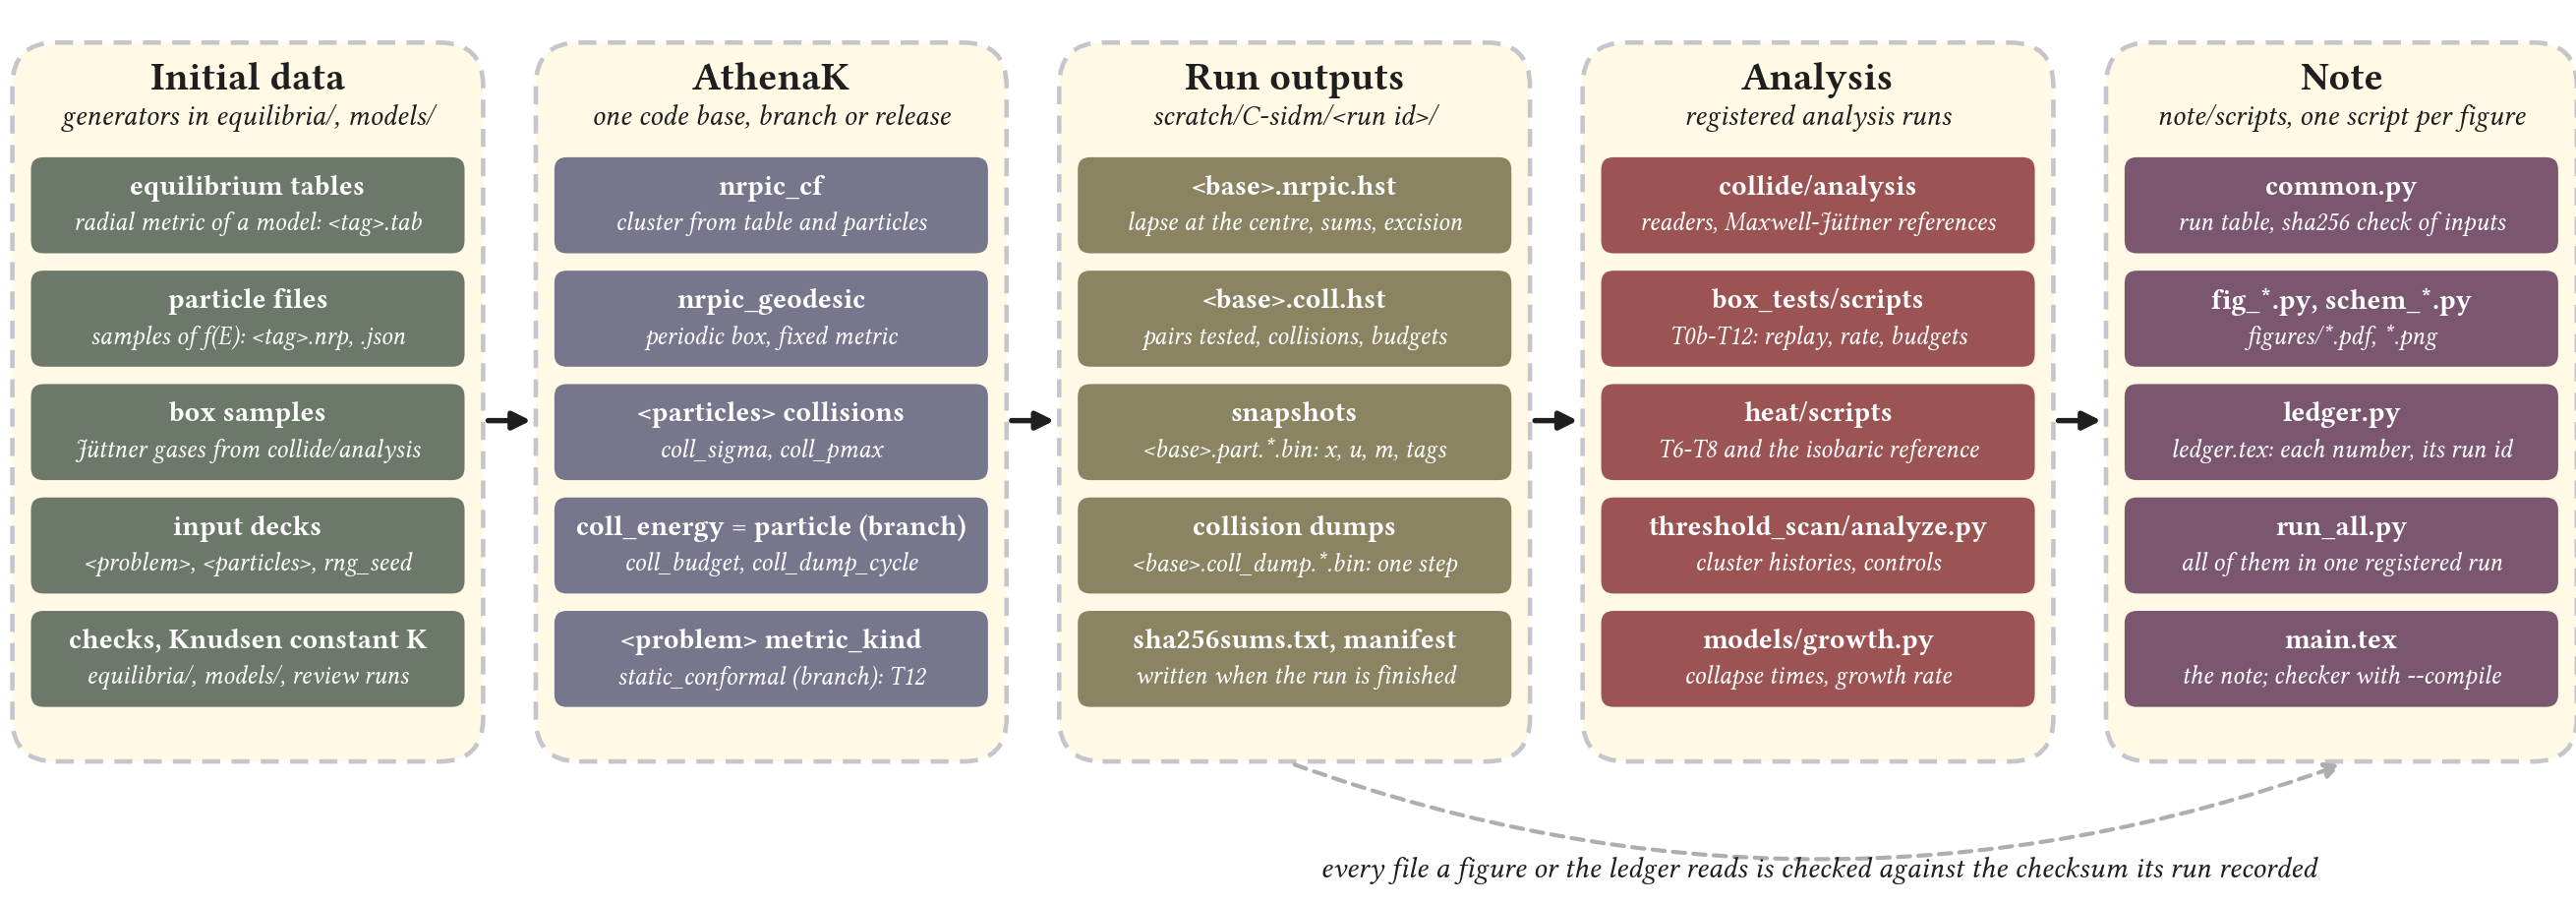
\includegraphics[width=\textwidth]{schem_dataflow.png}
\caption{Data flow behind this note: initial data, the code with the problem generators and options the track sets, the files a run writes, the analysis and the note's own scripts. Every step is a registered run that records the checksums of its outputs, and every file a figure or the ledger reads is checked against them.}
\label{fig:dataflow}
\end{figure*}

\bibliography{references}

\end{document}
